\section{Sítotisk}
-popis technologie depozice TLV past, parametry procesu, následné tepelné
zpracování vrstev

\subsection{Popis technologie depozice TLV past}
Nevakuový, relativně nenáročný způsob nanášení definovaného množství materiálu přes sítotiskové šablony na nosný substrát.

\textbf{Sítotiskový stroj:}
\begin{itemize}
\item Konstrukce pro uchycení rámu nesoucího šablonu
\item Přípravek pro uchycení substrátu
\item Pohyblivou část pro vedení stěrky
\end{itemize}

Rám s napnutým sítem, na němž je vytvořena šablona s tiskovým motivem je umístěn
v definované poloze vzhledem k držáku pro uchycení substrátu. S tím je spojen také mechanizmus pro uchycení stěrky. Stroj musí být robustní, a rovněž vedení stěrky musí být dostatečně tuhé.

Pasta nanesená na síto je protlačena přes síto stěrkou na substrát. Po odskoku síta
zůstane na substrátu požadovaný motiv.

Síta jsou tkaná z ocelových nebo z umělých vláken a vyznačují se pravidelnou osnovou
s definovanými parametry. Síto je umístěno nad substrátem ve vzdálenosti o, která se nazývá \textbf{odtrh (o)}. Tato vzdálenost se pohybuje kolem 0,8 mm, a musí být natolik dostatečná, aby byl zajištěn pružný odskok síta od substrátu po přechodu stěrky.

\textbf{Rámeček} (hliník, plast, textgumoid) - funkcí je udržet napnutí síťoviny v potřebném místě\\
\textbf{Tkanina} (nerez, polyester, polyamid) - funkcí je udržet napnutí síťoviny v potřebném místě
\begin{figure}[h]
   \begin{center}
     \includegraphics[scale=0.6]{images/Sitotisk.png}
   \end{center}
   \caption{Princip nanášení sítotiskem}
\end{figure}
\newpage

\subsection{Parametry procesu}
\begin{figure}[h]
   \begin{center}
     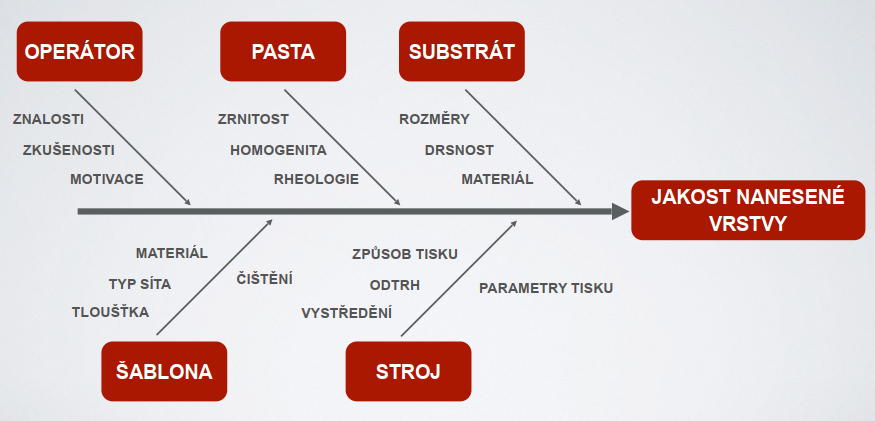
\includegraphics[scale=0.6]{images/Faktory.png}
   \end{center}
   \caption{Faktory působící v průběhu tisku}
\end{figure}

\subsubsection{Síto a jeho parametry}
\textbf{Rámeček} (hliník, plast, textgumoid) - funkcí je udržet napnutí
síťoviny v potřebném místě

\textbf{Tkanina} (nerez, polyester, polyamid) - funkcí je udržet napnutí síťoviny v potřebném místě

\textbf{Ovrstvení} - vytváří požadovaný tiskový motiv

\textbf{Vazba tkaniny} - (plane wave, twill wave, panama wave)

\textbf{Počet ok} – (hustota tkaniny), n [n/cm], určuje počet ok na cm nebo palec (Hrubá síta – 50 ok/cm, Jemná síta 155 ok/cm
\begin{equation}
n = \frac{10}{w+d}
\end{equation}

\begin{figure}[h]
   \begin{center}
     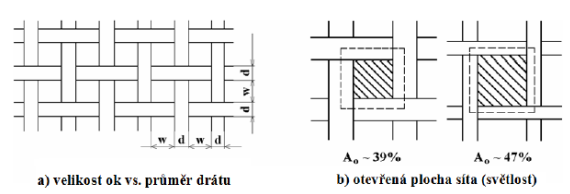
\includegraphics[scale=0.6]{images/Sito.png}
   \end{center}
   \caption{Parametry síta}
\end{figure}

\textbf{Průměr vlákna }– (tloušťka tkaniny → definuje výšku nanesené vrstvy)

\textbf{Světlost síta:} otevřená plocha síta
Materiály: nerezová ocel nebo polyester

Tisková plocha nesmí být příliš velká. V opačném případě by byla přítlačná
síla těrky neúměrně velká. Běžně by tisková plocha neměla přesahovat 2/3 plochy síta.

\begin{figure}[h]
   \begin{center}
     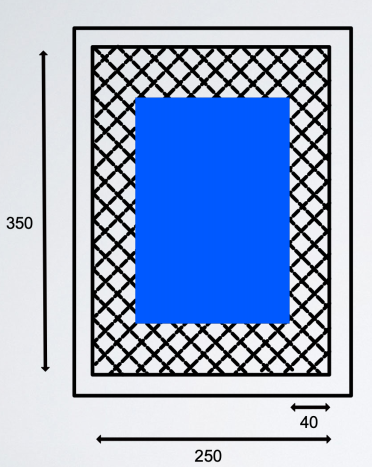
\includegraphics[scale=0.6]{images/Sito2.png}
   \end{center}
   \caption{Efektivní plocha síta}
\end{figure}

\textbf{Přímá sítotisková šablona} je vytvořena nanesením světlocitlivé emulze na
síťovinu(vtlačena do ok), na kterou je pomocí fotocesty přenesen požadovaný
motiv. Jeden ze způsobů nanášení je pomocí korýtka s fototocitlivou emulzí – realizuje se několik vrstev

\textbf{Nepřímá šablona} - v případě nepřímé sítotiskové šablony se její realizace
odehrává mimo samotné síto(motiv vytvořen na fólii) a tato je na něj
následně upevněna.

\begin{figure}[h]
   \begin{center}
     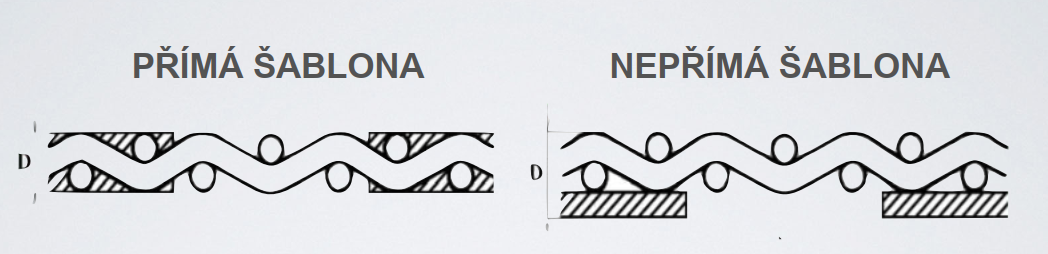
\includegraphics[scale=0.6]{images/Sablona.png}
   \end{center}
   \caption{Přímá a nepřímá šablona}
\end{figure}

\subsection{Tepelné zpracování}
Po nanesení tlustovrstvových materiálů na keramický substrát následuje po zasušení a
vyrovnání nanesené vrstvy při pokojové teplotě (min 15 min)-leveling, jejich teplotní zpracování, krátce nazývané výpal nebo sintrace. Tato operace probíhá v průtahové peci s definovaným teplotním profilem, kde dochází k tvorbě vlastní struktury.

Běžná doba výpalu se pohybuje kolem 50 minut a teplota žárového pásma je kolem 800 $^{\circ}$C podle druhu vypalované pasty. Nejrozšířenější je atmosféra vzduchová, ale pro materiály, které mají sklon k oxidaci, je třeba používat ochranou atmosféru,
například dusíkovou.

V průběhu výpalu dochází k chemické reakci směsí pasty a k vytváří spojení
vrstvy se substrátem a na povrchu se formuje aktivní struktura. Vypálená vrstva je tvrdá a odolná vůči mechanickým a chemickým vlivům.

\textbf{Sušení} - teplota se pohybuje od 70 do 150 $^{\circ}$C, doba sušení 15 až 30 minut. Dochází k úniku organických ředidel
těkavého charakteru z nanesené pasty.
\textbf{Zóna předehřívací} – teplota kolem 350 $^{\circ}$C, dochází k odpaření zbylých stop organických rozpouštědel, vyhořívá filmotvorný materiál

\textbf{Zóna vypalovací} – teplota 850 $^{\circ}$C, začíná tvorba slitin a slinování funkčních složek pasty, probíhají důležité chemické reakce ovlivňující výsledné vlastnosti pasty

\textbf{Zóna chladící} – dochází k ochlazování substrátů postupně až na teplotu okolí, tuhne roztavená skelná fáze ve vrstvě.

\begin{figure}[h]
   \begin{center}
     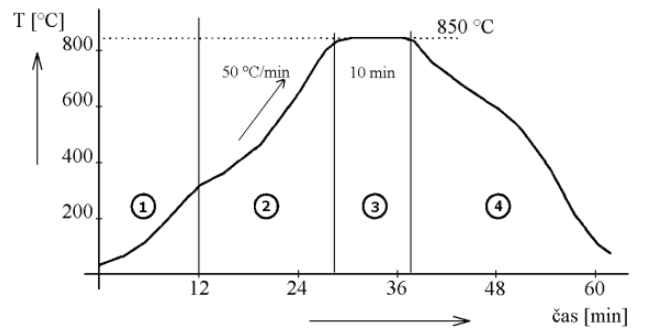
\includegraphics[scale=0.6]{images/Vypal.png}
   \end{center}
   \caption{Výpal TLV}
\end{figure}

\begin{figure}[h]
   \begin{center}
     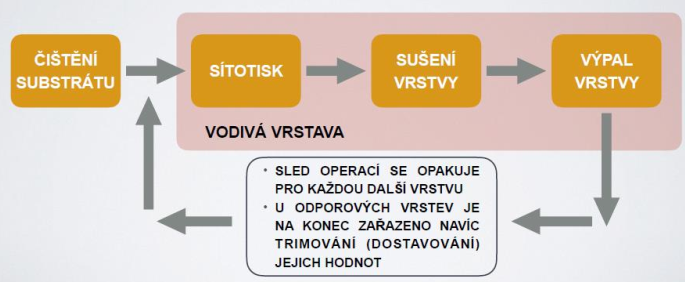
\includegraphics[scale=0.6]{images/Operace.png}
   \end{center}
   \caption{Sled operací u TLV}
\end{figure}



